\chapter{\textit{Modelagem Dinâmica}}

\section{Modelagem do Quadricóptero}
Um quadricóptero é um tipo de veículo aéreo não tripulado (VANT), caracterizado por possuir quatro rotores, que podem ser dispostos em diversas configurações. O Parrot Mambo, utilizado neste trabalho, possui uma configuração em X, com cada rotor podendo variar sua velocidade e direção de giro de forma independente.

Para estudar as características dinâmicas e o sistema de controle deste quadrirrotor, é necessário compreender como as forças que interagem com o corpo se relacionam. A análise dinâmica de um drone pode ser dividida em: dinâmica de corpo rígido, dinâmica translacional, cinemática e dinâmica de atitude, forças atuantes sobre o corpo, e controle. Neste capítulo, será apresentada essa análise.

\subsection{Configurações do Quadricóptero}
O Parrot Mambo é um quadricóptero composto por 4 atuadores (conjunto motor e hélice), controlados individualmente para gerar empuxo. Dois dos motores giram no sentido horário e dois no sentido anti-horário, de forma a equilibrar o momento resultante em torno do centro de massa, prevenindo rotações indesejadas.

Este estudo considera a configuração em 'X', que apresenta um desempenho superior (cerca de 30\%) em relação à configuração em '+' para os movimentos de rolagem e arfagem (Niemiec e Gandhi, 2014). Independentemente da configuração, o quadricóptero possui 6 graus de liberdade, sendo três para a translação nos eixos \(X\), \(Y\), \(Z\), e três para a rotação nos ângulos de Euler: rolagem (\(\phi\)), arfagem (\(\theta\)) e guinada (\(\psi\)).

Entretanto, o quadricóptero é subatuado, pois possui apenas quatro atuadores. Isso implica que ele não pode controlar diretamente todos os seus movimentos, como transladar lateralmente sem antes rotacionar. Para superar essa limitação, ele combina rotações e empuxo.

\subsection{Sistemas de Coordenadas}
Para a modelagem dinâmica de um quadricóptero, consideram-se o sistema de coordenadas inercial $\boldsymbol{\vec{I}} = \{\boldsymbol{\vec{X}}, \boldsymbol{\vec{Y}}, \boldsymbol{\vec{Z}}\}$, fixo no espaço, e o sistema de coordenadas do corpo $\boldsymbol{\vec{B}} = \{\boldsymbol{\vec{X_L}}, \boldsymbol{\vec{Y_L}}, \boldsymbol{\vec{Z_L}}\}$, que se move junto ao quadricóptero.

\begin{figure}[H]
	\centering
	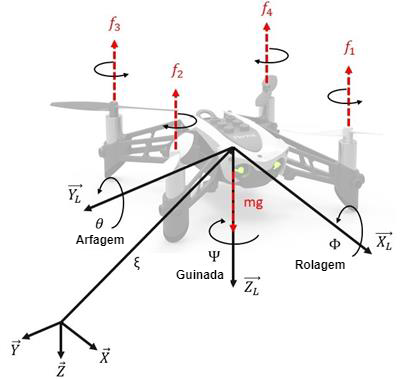
\includegraphics[width=0.6\textwidth]{coordinate-system.png}
	\caption{Representação do sistema de referência inercial e do sistema centralizado no corpo do drone. Fonte: Adaptado de Zaraza Espinosa e Buitrago Galvan (2023).}
	\label{fig:coordinate-system}
\end{figure}

\subsection{Matrizes de Rotação}
Agora que os sistemas de referência estão definidos, é necessário relacionar o sistema de referência inercial (\(\boldsymbol{\vec{I}}\)) com o sistema de referência do corpo (\(\boldsymbol{\vec{B}}\)) por meio da matriz de rotação \(R_{bi}\). Essa matriz é obtida através de três rotações sucessivas ao longo dos eixos do sistema inercial (sequência \(x\)-\(y\)-\(z\)):

\[
	R_{bi}(\phi,\theta,\psi) = R_z(\psi) R_y(\theta) R_x(\phi)
\]

\[
= \begin{bmatrix}
	\cos \theta \cos \psi & \sin \phi \sin \theta \cos \psi - \cos \phi \sin \psi & \cos \phi \sin \theta \cos \psi + \sin \phi \sin \psi \\
	\cos \theta \sin \psi & \sin \phi \sin \theta \sin \psi + \cos \phi \cos \psi & \cos \phi \sin \theta \sin \psi - \sin \phi \cos \psi \\
	-\sin \theta & \sin \phi \cos \theta & \cos \phi \cos \theta
\end{bmatrix}
\tag{1}
\]

\section{Movimentos do Quadricóptero}
Agora que discutimos as características e configurações do quadricóptero, podemos descrever os movimentos que ele realiza, associados aos seus 6 graus de liberdade. Cada movimento está relacionado a uma combinação de empuxo gerado pelos atuadores e rotações controladas, compensando as limitações de ser subatuado.

\subsection{Movimento de Rolagem (Roll - $\phi$)}
A rotação em torno do eixo longitudinal (\(X\)) do quadricóptero, chamada rolagem, ocorre quando os motores de um lado geram mais empuxo do que os motores do lado oposto, inclinando lateralmente o quadricóptero.

\begin{figure}[H]
	\centering
	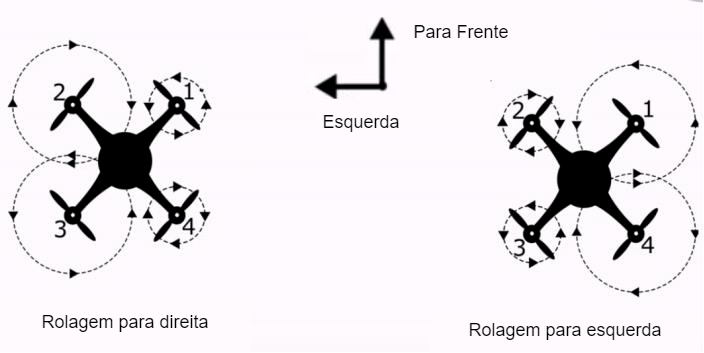
\includegraphics[width=0.8\textwidth]{rolagem-motores.png}
	\caption{Movimento de Rolagem em um quadricóptero com configuração em 'X' (Ceppi, 2020).}
	\label{fig:roll_maneuver}
\end{figure}

\begin{figure}[H]
	\centering
	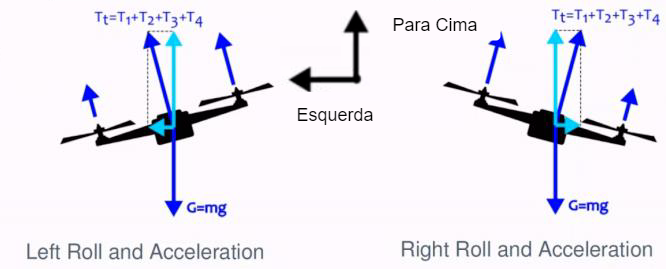
\includegraphics[width=0.8\textwidth]{rolagem-movimento.png}
	\caption{Balanço das forças durante a manobra de Rolagem (Ceppi, 2020).}
	\label{fig:roll_maneuver_forces}
\end{figure}

\subsection{Movimento de Arfagem (Pitch - $\theta$)}
A arfagem corresponde à rotação em torno do eixo lateral (\(Y\)), inclinando o quadricóptero para frente ou para trás. Esse movimento resulta do diferencial de empuxo entre os motores dianteiros e traseiros.

\begin{figure}[H]
	\centering
	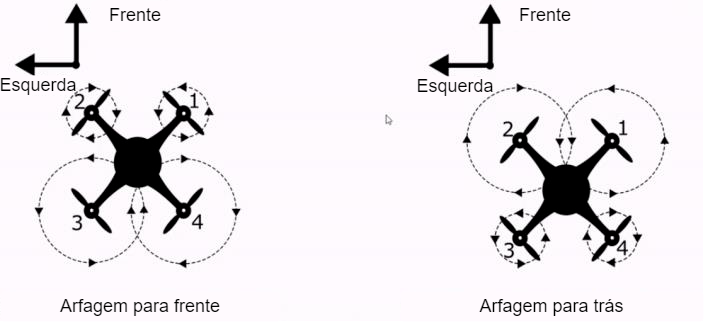
\includegraphics[width=0.8\textwidth]{arfagem-motores.png}
	\caption{Movimento de Arfagem em um quadricóptero com configuração em 'X' (Ceppi, 2020).}
	\label{fig:pitch_maneuver}
\end{figure}

\begin{figure}[H]
	\centering
	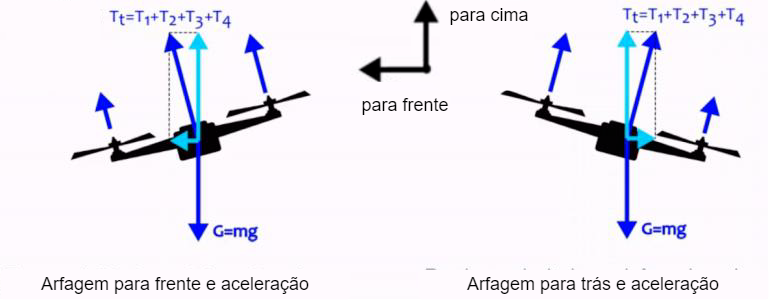
\includegraphics[width=0.8\textwidth]{arfagem-movimento.png}
	\caption{Balanço das forças durante a manobra de Arfagem (Ceppi, 2020).}
	\label{fig:pitch_maneuver_forces}
\end{figure}

\subsection{Movimento de Guinada (Yaw - $\psi$)}
A guinada refere-se à rotação em torno do eixo vertical (\(Z\)), que altera a direção do quadricóptero. Isso é conseguido ao variar as rotações dos motores no sentido horário e anti-horário, criando um momento resultante que gira o quadricóptero.

\begin{figure}[H]
	\centering
	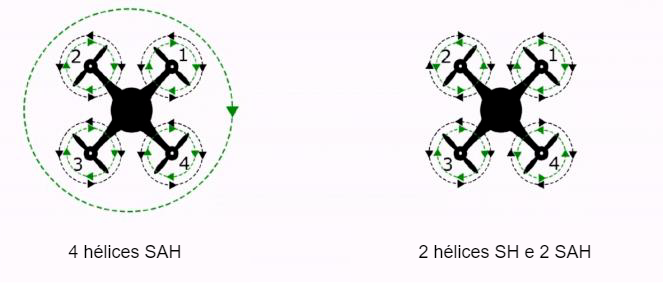
\includegraphics[width=0.8\textwidth]{guinada-motores-movimento.png}
	\caption{Balanço dos torques durante a guinada (Ceppi, 2020).}
	\label{fig:yaw_torques}
\end{figure}

\begin{figure}[H]
	\centering
	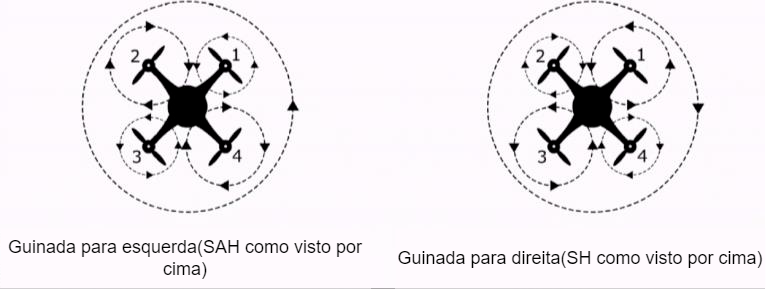
\includegraphics[width=0.8\textwidth]{guinada-movimento.png}
	\caption{Manobra de Guinada e balanço dos torques (Ceppi, 2020).}
	\label{fig:yaw_maneuver_torques}
\end{figure}

\subsection{Movimentos de Translação}
Os movimentos de translação são alcançados pela combinação das rotações já descritas:

\begin{itemize}
	\item \textbf{Translação no eixo \(X\) (lateral):} Consequência da inclinação em rolagem.
	\item \textbf{Translação no eixo \(Y\) (longitudinal):} Resulta da inclinação em arfagem.
	\item \textbf{Translação no eixo \(Z\) (vertical):} Controlada diretamente pela força de empuxo dos quatro atuadores.
\end{itemize}

Os movimentos de translação e rotação são coordenados pelo sistema de controle do quadricóptero, que supera as limitações do sistema subatuado ao combinar rotações e empuxo. Isso será detalhado no algoritmo de mistura dos motores.

As equações que governam o controle dos motores são expressas da seguinte forma:

\begin{align}
	\text{Motor}_{\text{frente-direita}} &= \text{Cmd}_{\text{empuxo}} + \text{Cmd}_{\text{guinada}} + \text{Cmd}_{\text{arfagem}} + \text{Cmd}_{\text{rolagem}} \tag{2} \\
	\text{Motor}_{\text{frente-esquerda}} &= \text{Cmd}_{\text{empuxo}} - \text{Cmd}_{\text{guinada}} + \text{Cmd}_{\text{arfagem}} - \text{Cmd}_{\text{rolagem}} \tag{3} \\
	\text{Motor}_{\text{trás-direita}} &= \text{Cmd}_{\text{empuxo}} - \text{Cmd}_{\text{guinada}} - \text{Cmd}_{\text{arfagem}} + \text{Cmd}_{\text{rolagem}} \tag{4} \\
	\text{Motor}_{\text{trás-esquerda}} &= \text{Cmd}_{\text{empuxo}} + \text{Cmd}_{\text{guinada}} - \text{Cmd}_{\text{arfagem}} - \text{Cmd}_{\text{rolagem}} \tag{5}
\end{align}

\section{Modelo Dinâmico Completo do Quadricóptero}
Após discutirmos a configuração, os sistemas de coordenadas e os movimentos básicos do quadricóptero, podemos avançar para o desenvolvimento do modelo dinâmico completo. O objetivo desta seção é descrever as equações que governam tanto a translação quanto a rotação do quadricóptero em relação aos sistemas de coordenadas definidos.

\subsection{Dinâmica Translacional}
A dinâmica translacional do quadricóptero é descrita pela Segunda Lei de Newton, que estabelece que a força resultante sobre um corpo é igual à massa do corpo multiplicada pela aceleração de seu centro de massa. No referencial inercial, as forças atuantes incluem o empuxo gerado pelos motores e as forças aerodinâmicas de arrasto. Essas forças, inicialmente no referencial do corpo, precisam ser transformadas para o referencial inercial usando as matrizes de rotação. A Tabela \ref{tab:termos_dinamica_translacional} resume os termos utilizados nas equações.

\begin{table}[H]
	\centering
	\begin{tabular}{|c|l|}
		\hline
		\textbf{Símbolo}  & \textbf{Descrição} \\ \hline
		$m$               & Massa total do quadricóptero \\ \hline
		$x_i, y_i, z_i$   & Coordenadas do centro de massa no referencial inercial \\ \hline
		$\ddot{x_i}, \ddot{y_i}, \ddot{z_i}$ & Acelerações do quadricóptero nas direções \(x_i\), \(y_i\) e \(z_i\) \\ \hline
		$T_i$             & Empuxo gerado pelo \(i\)-ésimo motor \\ \hline
		$\sum_{i=1}^{4} T_i$ & Empuxo total gerado pelos quatro motores \\ \hline
		$\theta$          & Ângulo de arfagem (pitch) \\ \hline
		$\phi$            & Ângulo de rolagem (roll) \\ \hline
		$g$               & Aceleração da gravidade \\ \hline
		$R_{ib}$          & Matriz de rotação do referencial do corpo para o inercial \\ \hline
	\end{tabular}
	\caption{Descrição dos termos utilizados nas equações da dinâmica translacional.}
	\label{tab:termos_dinamica_translacional}
\end{table}

Aplicando a Segunda Lei de Newton, a equação do movimento translacional no referencial inercial é dada por:

\[
m \begin{bmatrix}
\ddot{x_i} \\
\ddot{y_i} \\
\ddot{z_i}
\end{bmatrix} = R_{ib}
\begin{bmatrix}
0 \\
0 \\
\sum_{i=1}^{4} T_i
\end{bmatrix}
- m
\begin{bmatrix}
0 \\
0 \\
g
\end{bmatrix}
\tag{6}
\]

Aqui, o termo à esquerda representa a força total gerada pelos motores, transformada para o referencial inercial, e o termo à direita é a força da gravidade, atuando na direção \(z_i\). Ignorando o arrasto aerodinâmico, a força de empuxo \(T_i\), aplicada ao longo do eixo \(z_b\), é transformada para o referencial inercial usando a matriz de rotação \(R_{ib}\):

\[
\mathbf{T} = R_{ib} \begin{bmatrix} 
0 \\
0 \\
\sum_{i=1}^{4} T_i 
\end{bmatrix}
=
\begin{bmatrix} 
-\sin\theta \sum_{i=1}^{4} T_i \\
\sin\phi \cos\theta \sum_{i=1}^{4} T_i \\
\cos\phi \cos\theta \sum_{i=1}^{4} T_i
\end{bmatrix}
\tag{7}
\]

Combinando os termos de empuxo e gravidade, obtemos:

\[
m \frac{d^2}{dt^2} \begin{bmatrix} 
x_i \\ 
y_i \\ 
z_i 
\end{bmatrix}
=
\begin{bmatrix} 
-\sin\theta \sum_{i=1}^{4} T_i \\
\sin\phi \cos\theta \sum_{i=1}^{4} T_i \\
\cos\phi \cos\theta \sum_{i=1}^{4} T_i
\end{bmatrix}
- m \begin{bmatrix}
0 \\
0 \\
g
\end{bmatrix}
\tag{8}
\]

Explicando as componentes das equações individuais de translação:

\[
\ddot{x_i} = -\frac{T_t}{m} \sin\theta
\tag{9}
\]

\[
\ddot{y_i} = \frac{T_t}{m} \sin\phi \cos\theta
\tag{10}
\]

\[
\ddot{z_i} = \frac{T_t}{m} \cos\phi \cos\theta - g
\tag{11}
\]

onde:

- \(T_t = \sum_{i=1}^{4} T_i\) é o empuxo total gerado pelos motores.

\subsection{Dinâmica Rotacional}
A dinâmica rotacional é descrita pela equação de movimento angular:

\[
\vec{M} = \frac{d\vec{H}}{dt}
\tag{12}
\]

O momento angular total \(\vec{H}\) é dado por:

\[
\vec{H} = \mathbf{I} \vec{\omega}
\tag{13}
\]

onde \(\mathbf{I}\) é o tensor de inércia e \(\vec{\omega}\) é o vetor de velocidade angular. Em um drone simétrico, o tensor de inércia é diagonal:

\[
\mathbf{I} = \begin{pmatrix}
I_{xx} & 0 & 0 \\
0 & I_{yy} & 0 \\
0 & 0 & I_{zz}
\end{pmatrix}
\tag{14}
\]

Aplicando a derivada vetorial à equação \(\vec{M} = \frac{d\vec{H}}{dt}\), temos:

\[
\vec{M} = \mathbf{I} \frac{d\vec{\omega}}{dt} + \vec{\omega} \times (\mathbf{I} \vec{\omega})
\tag{15}
\]

Explicando as componentes dos momentos em cada eixo:

\[
M_x = I_{xx} \ddot{\phi} + (I_{zz} - I_{yy}) \dot{\theta} \dot{\psi}
\tag{16}
\]

\[
M_y = I_{yy} \ddot{\theta} + (I_{xx} - I_{zz}) \dot{\phi} \dot{\psi}
\tag{17}
\]

\[
M_z = I_{zz} \ddot{\psi} + (I_{yy} - I_{xx}) \dot{\phi} \dot{\theta}
\tag{18}
\]

As acelerações angulares são, portanto:

\[
\ddot{\phi} = \frac{1}{I_{xx}} \left( M_x - (I_{zz} - I_{yy}) \dot{\theta} \dot{\psi} \right)
\tag{19}
\]

\[
\ddot{\theta} = \frac{1}{I_{yy}} \left( M_y - (I_{xx} - I_{zz}) \dot{\phi} \dot{\psi} \right)
\tag{20}
\]

\[
\ddot{\psi} = \frac{1}{I_{zz}} \left( M_z - (I_{yy} - I_{xx}) \dot{\phi} \dot{\theta} \right)
\tag{21}
\]
